\documentclass[10pt]{article}
\usepackage{times}
\usepackage{graphicx}
\usepackage{hyperref}
\hypersetup{colorlinks,breaklinks,
            urlcolor=[rgb]{0,0,1},
            citecolor=[rgb]{0,0,1},
            linkcolor=[rgb]{0,0,01}}
\usepackage{fullpage}
\setlength{\parindent}{0em}
\setlength{\parskip}{1em}

\begin{document}
% Title Space
\section*{\centering \LARGE \textsc{Independent Study Proposal}}
%\subsection*{\centering \large \textit{Rahul Krishna}}

% Abstract
\subsection*{Abstract}
This independent study aims to explore the application of multidimensional 
prediction systems in predicting the defects in unseen data. The study proposes 
the use of contrast sets as a planner in order to help understand what changes 
are to be made to mitigate the defects. The efficacy of these changes will 
then be evaluated using one of several established predictors in software 
defect prediction, such as 
random forest, CART, logistic regression, and so on, as suggested by 
\cite{lessmann}. The 
system 
consists of two 
phases -- Planning and Prediction. A flow chart of the proposed system is shown 
in Fig. \ref{fig1}. 
\begin{figure}[h!]
\centering
\begin{minipage}{0.7\textwidth}
	\centering
	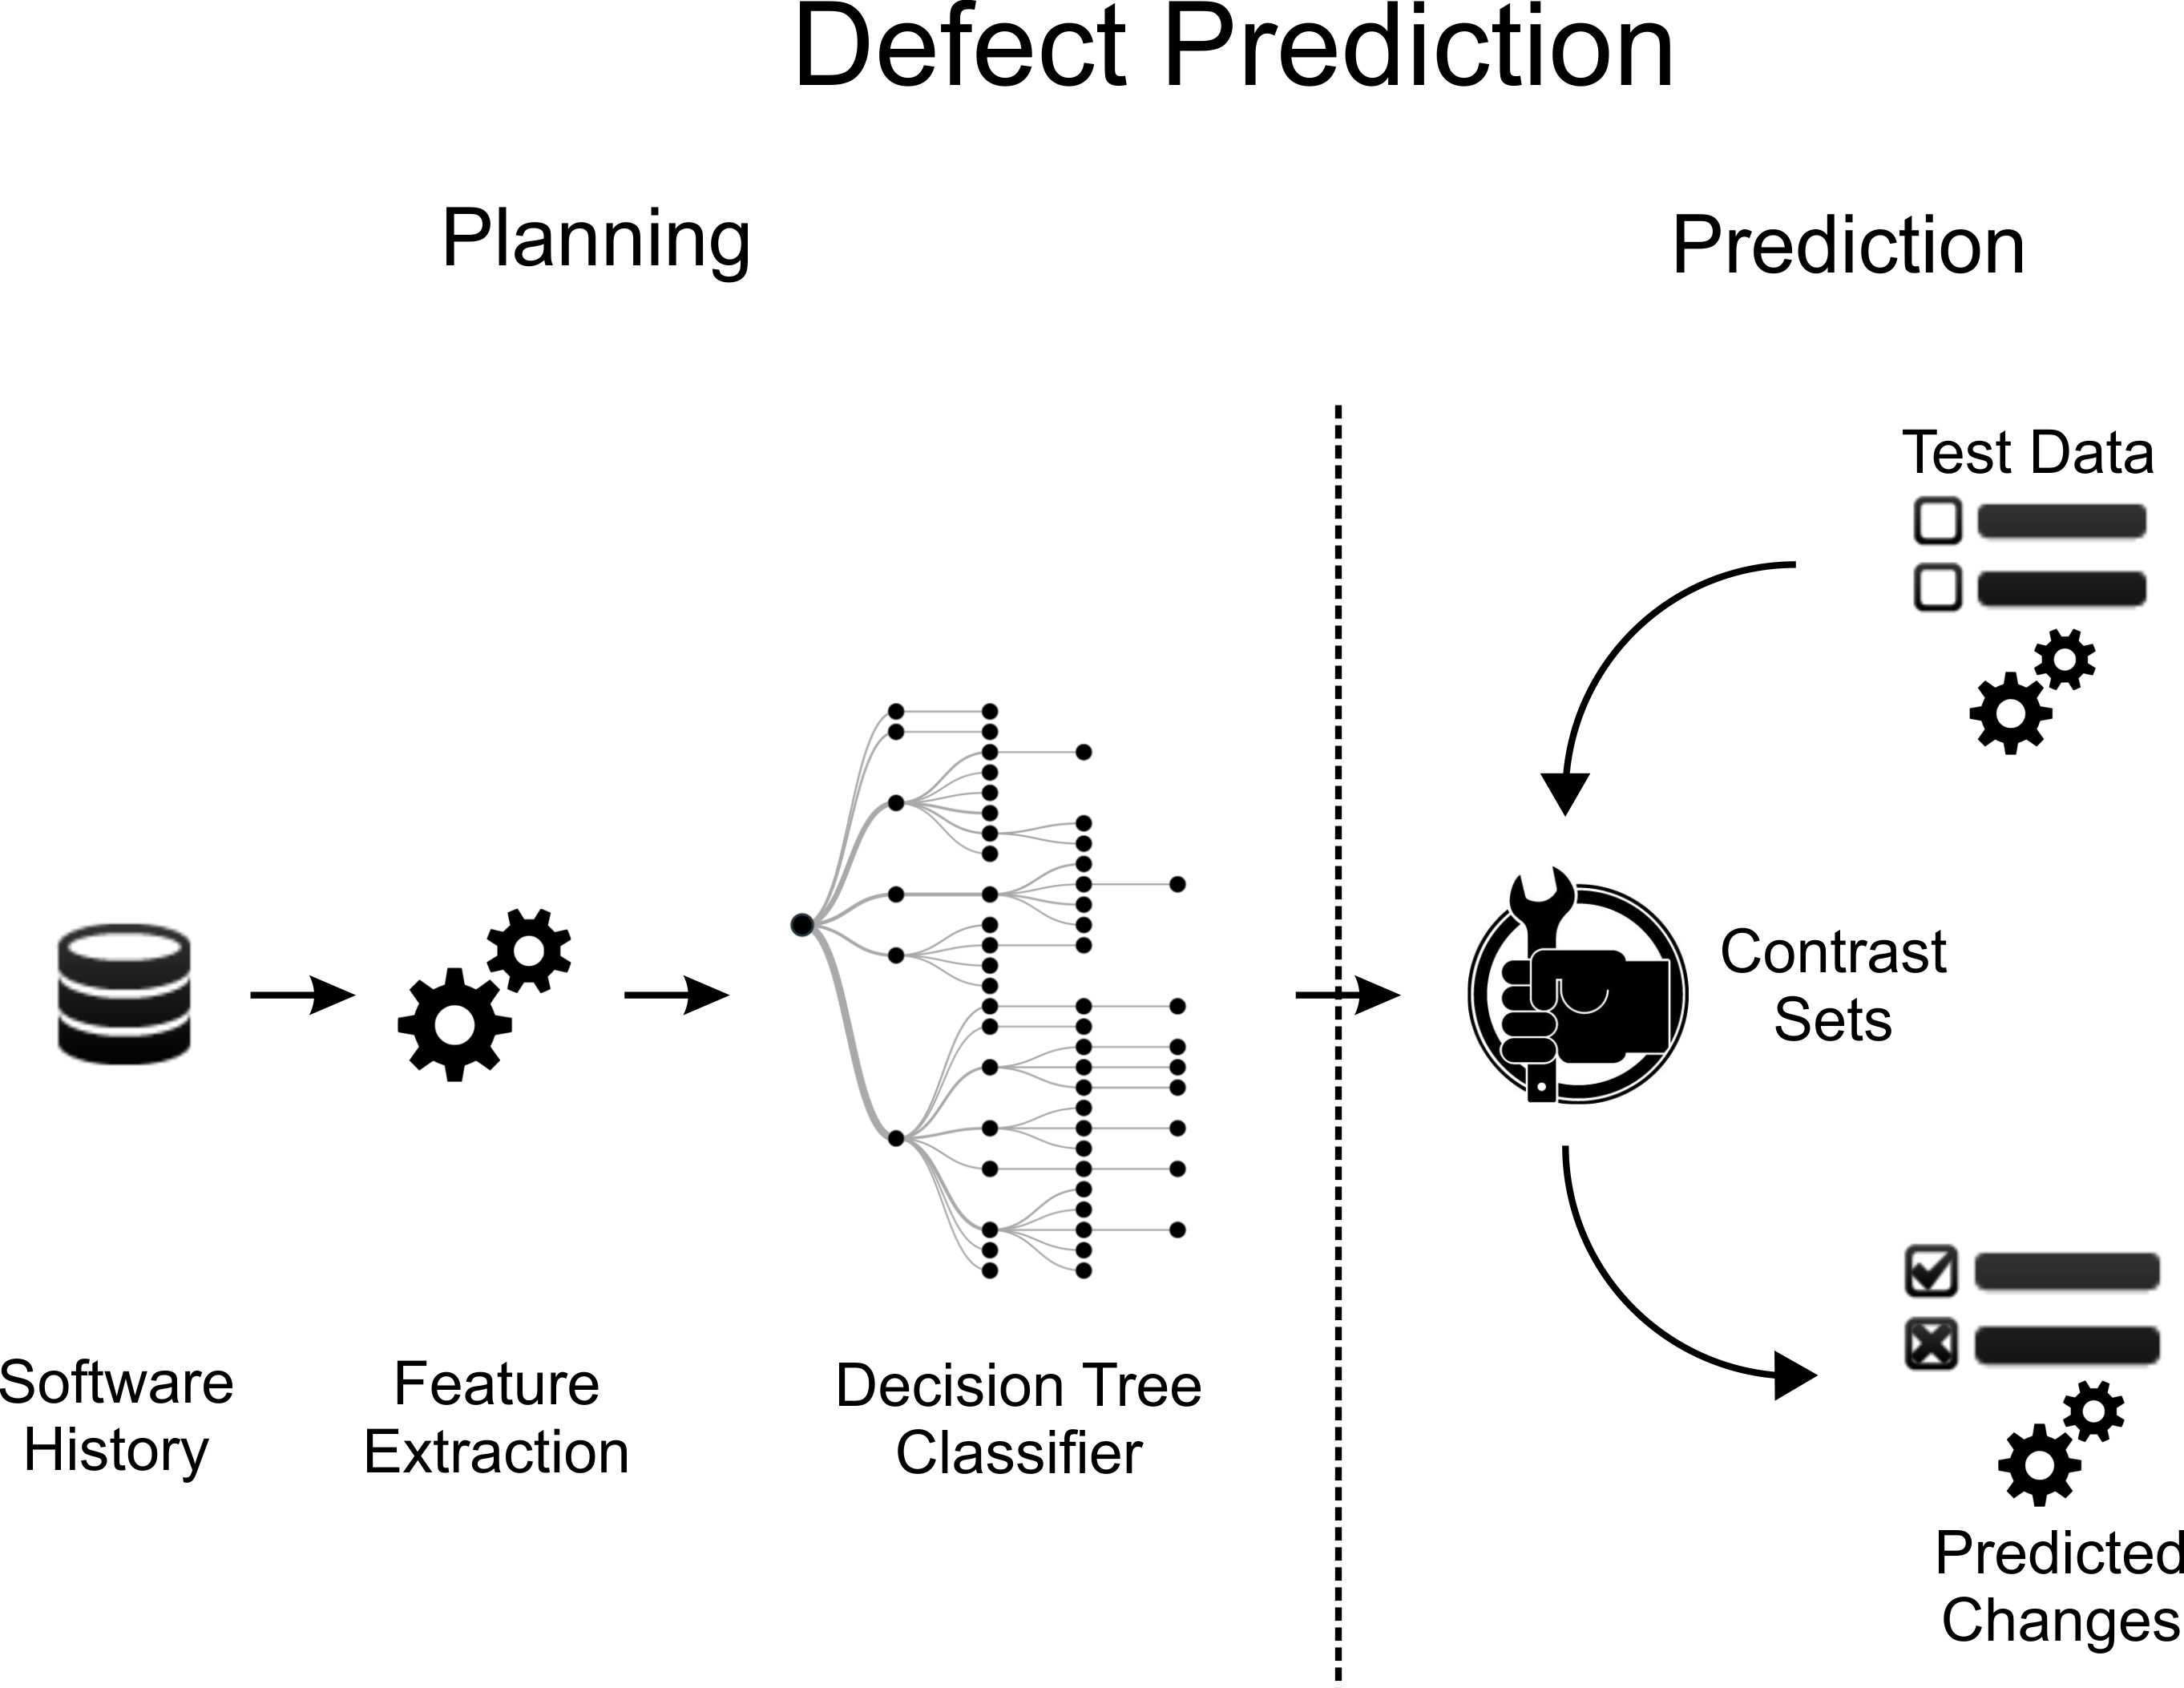
\includegraphics[width = \linewidth]{flowchart}
	\caption{Flowchart of the proposed defect prediction system.}
	\label{fig1}
\end{minipage}
\end{figure}

\begin{figure}[h!]
\begin{minipage}{0.5\textwidth}
The planning phase uses training data with recursive 
\textit{FASTMAP} 
clustering to create a decision tree. For a test data, we generate contrast 
sets 
to indicate changes that needs to be made to in order to reduce defects. The 
prediction phase implements these changes and predicts the defects in the 
modified data. We would like to study the distribution of defects in the 
modified 
data set compared to the raw test dataset and make appropriate improvements to 
the planning system. Much of the preliminary work was carried out fall 2014 and 
thus we anticipate early success; We plan on evaluating our techniques on 10 
defect datasets that have be gathered in the 
\href{https://github.com/rahlk/Research/tree/master/Defects/Data}{Promise} 
repository. Figure \ref{fig2} lists characeteristics of the defect data sets 
\cite{fayola}.\\[-1cm]
\end{minipage} \hspace{0.01\linewidth}
\begin{minipage}{0.5\textwidth}
	\centering
	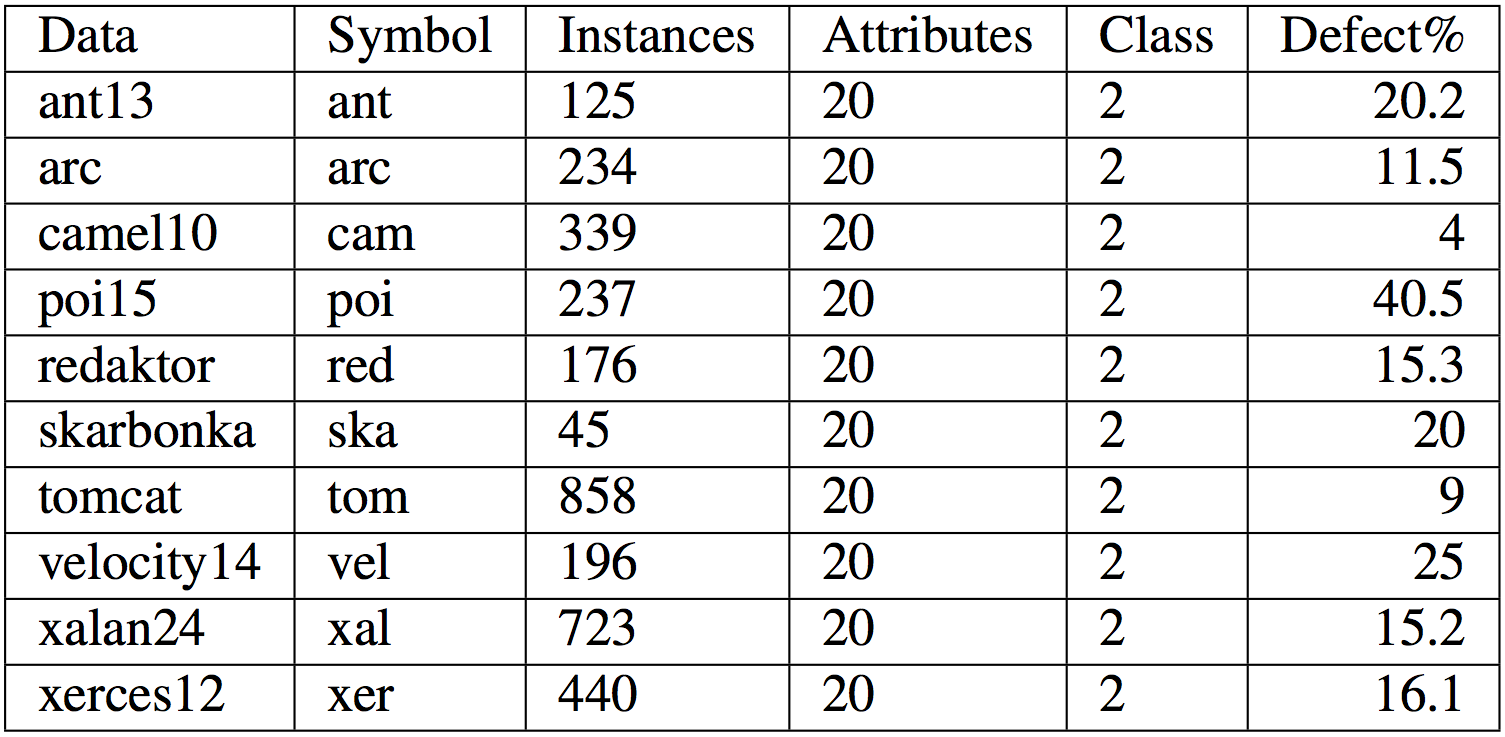
\includegraphics[width = \linewidth]{datasets}
	\caption{Defect Data Set Characteristics}
	\label{fig2}
\end{minipage}
\end{figure}
\begin{thebibliography}{10}
\bibitem{lessmann}
Lessmann, S.; Baesens, B.; Mues, C.; Pietsch, S., ``Benchmarking Classification 
Models for Software Defect Prediction: A Proposed Framework and Novel 
Findings,'' Software Engineering, IEEE Transactions on , vol.34, no.4, 
pp.485,496, July-Aug. 2008
doi: 10.1109/TSE.2008.35
\bibitem{fayola}
Peters, F.; Menzies, T., ``Privacy and utility for defect prediction: 
Experiments with MORPH,'' Software Engineering (ICSE), 2012 34th International 
Conference on , vol., no., pp.189,199, 2-9 June 2012
doi: 10.1109/ICSE.2012.6227194
\end{thebibliography}
\end{document}